\documentclass[11pt]{article}
\usepackage[a4paper,margin=2.2cm]{geometry}
\usepackage{amsmath,amssymb}
\usepackage{graphicx}
\usepackage{booktabs}
\usepackage{array}
\usepackage{float}
\usepackage{tikz}
\usetikzlibrary{decorations.pathreplacing}
\usepackage[hidelinks]{hyperref}
\graphicspath{{figures/}}
\setlength{\parskip}{0.5em}
\setlength{\parindent}{0pt}

\title{Background for slide 17: where the DPC gradient comes from and why it explodes}
\author{Binoy George}
\date{30 October 2026}

\begin{document}
\maketitle

Slide 17 (``Why: through the kink, the gradient explodes'') says that DPC training through a kinked surrogate fails because the gradient explodes, while the surrogate's prediction of the cost stays correct. This note builds the mathematics behind that statement from the chain rule up (Sections 1 to 12) and then reads the slide piece by piece (Section 13). Section 14 lists what the later theory work added.

\section{The question DPC needs answered}

DPC trains the controller's weights $\theta$ by gradient descent on the cost
\begin{equation}
L(\theta)=\frac1N\Big(\sum_{k=0}^{N-1}\big(Q x_k^2+R u_k^2\big)+Q_f x_N^2\Big),\qquad Q=5,\ R=0.1,\ Q_f=50,\ N=200,
\end{equation}
averaged over 1000 starts, where the states come from rolling the controller through the surrogate:
\begin{equation}
x_{k+1}=\hat F(x_k,u_k),\qquad u_k=\pi_\theta(x_k).
\end{equation}
Each training step needs $dL/d\theta$: if the weights change a tiny bit, how much does the cost change? Everything below is the chain rule written out step by step for this closed loop.

\section{What $\delta$ means}

Imagine two runs from the same start $x_0$. The original run uses weights $\theta$ and visits $x_0,x_1,x_2,\dots$ with inputs $u_0,u_1,\dots$. The nudged run uses $\theta+\delta\theta$, with $\delta\theta$ tiny, and visits $x_0,\ x_1+\delta x_1,\ x_2+\delta x_2,\dots$ with inputs $u_k+\delta u_k$. So $\delta x_k$ is ``nudged minus original'' at step $k$, and likewise $\delta u_k$ and $\delta L$. The gradient is the ratio $\delta L/\delta\theta$ in the limit $\delta\theta\to0$. Because $\delta\theta$ is tiny, every $\delta$ is tiny, and products of two $\delta$'s are dropped. That is what ``first order'' means.

\section{The plant step: where $\delta x_{k+1}=\hat J_x\,\delta x_k+\hat J_u\,\delta u_k$ comes from}

The model gives the next state from the current state and input. In the original and the nudged run:
\begin{align}
x_{k+1}&=\hat F(x_k,u_k),\\
x_{k+1}+\delta x_{k+1}&=\hat F(x_k+\delta x_k,\ u_k+\delta u_k).
\end{align}
The first-order Taylor expansion of a function of two variables is
\begin{equation}
\hat F(x+a,\,u+b)\approx \hat F(x,u)+\frac{\partial \hat F}{\partial x}\,a+\frac{\partial \hat F}{\partial u}\,b .
\end{equation}
Apply it with $a=\delta x_k$, $b=\delta u_k$ and subtract the original line:
\begin{equation}\label{eq:plant}
\delta x_{k+1}=\hat J_x(k)\,\delta x_k+\hat J_u(k)\,\delta u_k,\qquad
\hat J_x(k)=\frac{\partial \hat F}{\partial x}(x_k,u_k),\quad \hat J_u(k)=\frac{\partial \hat F}{\partial u}(x_k,u_k).
\end{equation}
In words: the change in the next state is the slope in $x$ times the change in $x$, plus the slope in $u$ times the change in $u$.

For the true plant $f(x,u)=1.03x+0.01u$ this is exact, with $\hat J_x=A=1.03$ and $\hat J_u=B=0.01$ at every step. For the surrogate, $\hat J_x(k)$ and $\hat J_u(k)$ are evaluated at the point $(x_k,u_k)$ the original run occupies at step $k$: they are exactly the slopes drawn on the kink maps (slides 5 to 7). Whenever the trajectory passes through the kink, the kinked slopes enter here. This is the only place where the model enters the gradient.

This is the same step as linearising a plant for LQR, $x^+\approx Ax+Bu$ around an operating point. The difference is that here the linearisation is taken around every point of the trajectory, so the slopes change with $k$. In control language, (\ref{eq:plant}) is the linear time-varying system along a trajectory, also called the sensitivity or variational equation.

\section{The controller step: where $\delta u_k=-K_k\,\delta x_k+(\partial\pi/\partial\theta)\,\delta\theta$ comes from}

The controller's output depends on two things: its weights and the state it sees. In the nudged run both differ, so the same Taylor step gives
\begin{equation}
\delta u_k=\frac{\partial \pi}{\partial x}(x_k)\,\delta x_k+\frac{\partial \pi}{\partial \theta}(x_k)\,\delta\theta .
\end{equation}
Define the controller's local feedback gain $K_k=-\partial\pi/\partial x$ at $x_k$. The minus sign follows the LQR convention $u=-Kx$: for that controller $K_k=K$. Then
\begin{equation}\label{eq:ctrl}
\delta u_k=-K_k\,\delta x_k+\frac{\partial \pi}{\partial \theta}(x_k)\,\delta\theta .
\end{equation}
The input changes for two reasons. Directly, because the weights changed (the second term). Through feedback, because earlier weight changes moved the state and the controller reacts to the moved state (the first term).

Example: for the simplest controller $u=-\theta x$, $\partial\pi/\partial\theta=-x_k$ and $K_k=\theta$.

\section{Combining the two: the closed-loop multiplier}

Substitute (\ref{eq:ctrl}) into (\ref{eq:plant}):
\begin{equation}\label{eq:closed}
\delta x_{k+1}=\underbrace{\big(\hat J_x(k)-\hat J_u(k)\,K_k\big)}_{m_k}\,\delta x_k\;+\;\underbrace{\hat J_u(k)\,\frac{\partial \pi}{\partial \theta}(x_k)\,\delta\theta}_{s_k}.
\end{equation}
The number $m_k=\hat J_x(k)-\hat J_u(k)K_k$ is the closed loop's slope: how a state error at step $k$ becomes a state error at step $k+1$ once the controller has reacted. On the true plant with the LQR gain $K=10.29$,
\begin{equation}
m=A-BK=1.03-0.01\times10.29=0.927,
\end{equation}
which is the closed-loop pole of the LQR slides. So $m_k$ is the local closed-loop pole read from the surrogate's slopes at step $k$. The term $s_k$ is the new change injected at step $k$ by the weight change.

\section{Unrolling the rule, one step at a time}

Section 5 gave one rule that links step $k$ to step $k+1$:
\begin{equation}\label{eq:rule}
\delta x_{k+1}=m_k\,\delta x_k+s_k .
\end{equation}
This section applies the rule over and over, to see what $\delta x_k$ looks like after many steps.

\subsection{The rule in words: a bank balance}

Read (\ref{eq:rule}) as a bank account. The balance is $\delta x_k$, the error in the state caused by the weight change. At every step two things happen, in this order:
\begin{enumerate}
\item The whole balance is multiplied by $m_k$. If $m_k<1$ this is a fee that shrinks it; if $m_k>1$ it is interest that grows it.
\item A new deposit $s_k$ is added. The deposit is the fresh change that the weight change causes at this step, through the controller's output.
\end{enumerate}
The account opens empty: the start $x_0$ is the same in both runs, so $\delta x_0=0$.

\subsection{The first three steps, written out}

Step 1. Use the rule with $k=0$ and $\delta x_0=0$:
\begin{equation}
\delta x_1=m_0\cdot0+s_0=s_0 .
\end{equation}
Step 2. Use the rule with $k=1$ and put in $\delta x_1=s_0$:
\begin{equation}
\delta x_2=m_1\,\delta x_1+s_1=m_1 s_0+s_1 .
\end{equation}
Step 3. Use the rule with $k=2$ and put in $\delta x_2=m_1 s_0+s_1$:
\begin{equation}
\delta x_3=m_2\,\delta x_2+s_2=m_2\,(m_1 s_0+s_1)+s_2=m_2 m_1 s_0+m_2 s_1+s_2 .
\end{equation}
Nothing new is happening in these lines: each is the previous one, multiplied by the next $m$, plus the next deposit.

\subsection{What happened to each deposit}

The table follows each deposit separately. A deposit made at one step is multiplied by every $m$ that comes after it.

\begin{center}
\begin{tabular}{llll}
\toprule
 & at step 1 & at step 2 & at step 3 \\
\midrule
deposit $s_0$ (made at step 0) & $s_0$ & $m_1 s_0$ & $m_2 m_1 s_0$ \\
deposit $s_1$ (made at step 1) & -- & $s_1$ & $m_2 s_1$ \\
deposit $s_2$ (made at step 2) & -- & -- & $s_2$ \\
\midrule
balance $\delta x_k$ (column sum) & $s_0$ & $m_1 s_0+s_1$ & $m_2m_1s_0+m_2s_1+s_2$ \\
\bottomrule
\end{tabular}
\end{center}

\subsection{The general pattern}

At step $k$, the balance is the sum of all deposits made so far, each multiplied by all the multipliers that came after it:
\begin{equation}\label{eq:sum}
\delta x_k=\sum_{j=0}^{k-1}\big(m_{k-1}\,m_{k-2}\cdots m_{j+1}\big)\,s_j .
\end{equation}
For the newest deposit ($j=k-1$) the bracket is empty and counts as 1, since it has not been multiplied yet. The oldest deposit ($j=0$) carries the longest product, $k-1$ multipliers.

\subsection{From $\delta x_k$ to the derivative}

Every deposit is proportional to the weight change: $s_j=\hat J_u(j)\,\frac{\partial\pi}{\partial\theta}(x_j)\,\delta\theta$. So $\delta x_k$ is proportional to $\delta\theta$, and dividing (\ref{eq:sum}) by $\delta\theta$ gives the derivative of the state with respect to the weights:
\begin{equation}\label{eq:product}
\frac{dx_k}{d\theta}=\sum_{j=0}^{k-1}\big(m_{k-1}\cdots m_{j+1}\big)\;\hat J_u(j)\,\frac{\partial\pi}{\partial\theta}(x_j).
\end{equation}
This is the product formula. Its message: the effect of a weight change on the state at step $k$ is a sum of contributions from all earlier steps, and the contribution from step $j$ is multiplied by every closed-loop multiplier between step $j$ and step $k$.

\section{A worked example}

True plant, controller $u=-\theta x$ with $\theta=10$, start $x_0=1$, nudge $\delta\theta=0.01$. Then:
\begin{itemize}
\item every multiplier is the same, $m=A-B\theta=1.03-0.01\times10=0.93$;
\item the deposit at step $k$ is $s_k=B\cdot\frac{\partial\pi}{\partial\theta}\cdot\delta\theta=0.01\times(-x_k)\times0.01$, so $s_0=-0.000100$, $s_1=-0.000093$, $s_2=-0.0000865$.
\end{itemize}

First, the balance step by step, compared with simply running both versions of the controller:

\begin{center}
\small
\begin{tabular}{rllll}
\toprule
$k$ & original $x_k$ & nudged $x_k$ & measured $\delta x_k$ & from the rule (\ref{eq:rule}) \\
\midrule
1 & 0.93 & 0.9299 & $-0.000100$ & $0.93\cdot0+(-0.000100)=-0.000100$ \\
2 & 0.8649 & 0.864714 & $-0.000186$ & $0.93\cdot(-0.000100)+(-0.000093)=-0.000186$ \\
3 & 0.804357 & 0.804098 & $-0.000259$ & $0.93\cdot(-0.000186)+(-0.0000865)=-0.000259$ \\
\bottomrule
\end{tabular}
\end{center}

Second, the same balance at step 3, split into its three deposits as in the table of Section 6.3:
\begin{align}
m_2 m_1 s_0&=0.93\times0.93\times(-0.000100)=-0.0000865,\\
m_2 s_1&=0.93\times(-0.000093)=-0.0000865,\\
s_2&=-0.0000865,
\end{align}
which add up to $-0.000259$. (Here the three contributions happen to be equal, because the state itself shrinks by the same factor 0.93 per step, so each later deposit is smaller by exactly the factor the earlier ones have been shrunk by.)

\section{From state changes to the change in cost}

\subsection{How a small change in $x$ changes $x^2$}

The cost is built from squares. If $x$ changes to $x+\delta x$,
\begin{equation}
(x+\delta x)^2-x^2=2x\,\delta x+(\delta x)^2\approx2x\,\delta x ,
\end{equation}
because $(\delta x)^2$ is tiny compared with $\delta x$. Example: $x=0.93$ and $\delta x=-0.0001$ change $x^2$ by $2\times0.93\times(-0.0001)=-0.000186$.

\subsection{Adding up over the run}

Apply this to every term of the cost:
\begin{equation}
\delta L\approx\frac1N\Big(\sum_{k=0}^{N-1}\big(2Qx_k\,\delta x_k+2Ru_k\,\delta u_k\big)+2Q_fx_N\,\delta x_N\Big),
\end{equation}
and divide by $\delta\theta$ to get $dL/d\theta$. Every $\delta x_k$ in this sum is the balance of Section 6, so the gradient is a sum of products of multipliers. Whatever those products do, the gradient does too.

Check over 200 steps on the true plant with $\theta=10.29$, $x_0=1$: this sum gives $dL/d\theta=2.00256\times10^{-5}$, and a finite difference (running $\theta\pm10^{-6}$ and comparing the costs) gives $2.00258\times10^{-5}$.

\subsection{What backpropagation does differently}

Backpropagation computes the same number in the opposite order. Instead of carrying $\delta x_k$ forward from the start, it starts at the end and carries backwards the quantity
\begin{equation}
p_k=\text{how much the cost from step $k$ onwards changes if $x_k$ is nudged by one unit.}
\end{equation}
At the last step $p_N=2Q_fx_N/N$. Going one step back, a nudge of $x_k$ changes the cost at step $k$ itself, and it also moves $x_{k+1}$ by $m_k$ times as much, which the later cost already prices at $p_{k+1}$:
\begin{equation}
p_k=\frac{2Qx_k-2Ru_kK_k}{N}+m_k\,p_{k+1}.
\end{equation}
The gradient is then $\frac{dL}{d\theta}=\sum_k\big(\frac{2Ru_k}{N}+\hat J_u(k)\,p_{k+1}\big)\frac{\partial\pi}{\partial\theta}(x_k)$. On the example above this gives the same $2.00256\times10^{-5}$. The backward pass multiplies by the same $m_k$, only from the other end, so it has the same products; it is preferred because one backward pass gives the derivative for all 12\,737 GRU weights at once.

\section{Multiplying many numbers}

\subsection{Repeated multiplication}

The products in (\ref{eq:product}) can contain up to 200 multipliers. Here is what happens when the same number is multiplied by itself:

\begin{center}
\begin{tabular}{lllllll}
\toprule
number of factors & 1 & 2 & 3 & 10 & 50 & 200 \\
\midrule
$0.93$ & 0.93 & 0.865 & 0.804 & 0.48 & 0.027 & $5\times10^{-7}$ \\
$1.13$ & 1.13 & 1.28 & 1.44 & 3.4 & 451 & $4\times10^{10}$ \\
$-1.95$ & $-1.95$ & 3.80 & $-7.41$ & $795$ & $3\times10^{14}$ & $10^{58}$ \\
\bottomrule
\end{tabular}
\end{center}

A multiplier a little below 1 makes old deposits vanish. A multiplier a little above 1 makes them grow without bound. A multiplier below $-1$ makes them grow while flipping sign every step.

\subsection{Logarithms turn products into sums}

The multipliers usually differ from step to step, so the product $m_1m_2\cdots m_N$ cannot be written as one number raised to a power. Logarithms solve this. This subsection derives, one step at a time, the identity
\begin{equation}\label{eq:lyap}
|m_1 m_2\cdots m_N|=e^{N\lambda},\qquad\text{where}\qquad \lambda=\frac1N\sum_{k=1}^{N}\log|m_k| .
\end{equation}
Throughout, $\log$ is the natural logarithm (base $e$).

\paragraph{Three facts used.}
\begin{itemize}
\item Fact 1: $\log$ and $e^{(\cdot)}$ undo each other. For any positive number $a$, $e^{\log a}=a$. Example: $\log 2=0.693$ and $e^{0.693}=2$.
\item Fact 2: the logarithm of a product is the sum of the logarithms: $\log(ab)=\log a+\log b$, and the same for any number of factors.
\item Fact 3: the size of a product is the product of the sizes: $|ab|=|a|\,|b|$.
\end{itemize}
The absolute values are needed because a logarithm is only defined for positive numbers, while multipliers can be negative (for example $-1.95$). The sign only tells whether the error flips; the size is what grows or shrinks.

\paragraph{The derivation in five steps.} Call the size of the product $P=|m_1m_2\cdots m_N|$.
\begin{enumerate}
\item By Fact 3, $P=|m_1|\,|m_2|\cdots|m_N|$, a product of positive numbers.
\item Take the logarithm of both sides and use Fact 2:
\begin{equation}
\log P=\log|m_1|+\log|m_2|+\dots+\log|m_N|=\sum_{k=1}^{N}\log|m_k| .
\end{equation}
\item The definition of $\lambda$ in (\ref{eq:lyap}) is this sum divided by $N$. Multiplying the definition by $N$ gives
\begin{equation}
\sum_{k=1}^{N}\log|m_k|=N\lambda .
\end{equation}
\item Steps 2 and 3 have the same left-hand sum, so
\begin{equation}
\log P=N\lambda .
\end{equation}
\item Undo the logarithm with Fact 1: $P=e^{\log P}=e^{N\lambda}$.
\end{enumerate}
That is (\ref{eq:lyap}). It is exact, not an approximation: $\lambda$ is defined precisely so that it holds.

\paragraph{A check with three numbers.} Take $m_1=0.93$, $m_2=1.13$, $m_3=-1.95$.

\begin{center}
\begin{tabular}{ll}
\toprule
direct product & $0.93\times1.13\times(-1.95)=-2.049$, so $P=2.049$ \\
logarithms of the sizes & $\log0.93=-0.0726$,\quad $\log1.13=+0.1222$,\quad $\log1.95=+0.6678$ \\
their sum & $0.7175$ \\
$\lambda$ (sum divided by $N=3$) & $0.2392$ \\
$e^{N\lambda}=e^{3\times0.2392}=e^{0.7175}$ & $2.049$, the same as $P$ \\
\bottomrule
\end{tabular}
\end{center}

\paragraph{What $\lambda$ means.} If every step multiplied by the same number $e^\lambda$, then after $N$ steps the total would be $e^\lambda\times e^\lambda\times\dots\times e^\lambda=e^{N\lambda}$. So $e^\lambda$ is the typical multiplier per step: the single constant multiplier that gives the same total after $N$ steps as the actual, varying ones. (It is the geometric mean of the $|m_k|$.) In the check above, $e^{0.2392}=1.2702$, and $1.2702\times1.2702\times1.2702=2.049$.

$\lambda$ is called the Lyapunov exponent. Negative $\lambda$ means $e^\lambda<1$: the product shrinks. Positive $\lambda$ means $e^\lambda>1$: the product grows exponentially with $N$.

\paragraph{Why the curves on slide 17 look straight.} The plot uses a logarithmic axis. By Step 2, the logarithm of the running product grows by $\log|m_k|$ at every step, so on a log axis the curve rises by $\log|m_k|$ per step, and over a stretch where the multipliers behave similarly it is a straight line whose slope is $\lambda$ (in natural-log units per step). In the middle panel of slide 17 the slope is about $0.39$ per step, a typical multiplier of $e^{0.39}=1.48$, and after 200 steps $e^{0.39\times200}=e^{78}\approx10^{34}$, which is where that curve ends.

Example: half of 200 steps with $m=0.93$ ($\log=-0.073$) and half with $m=1.13$ ($\log=+0.122$). The average is $\lambda=+0.025$, so the product is $e^{200\times0.025}\approx143$: a mixture can grow overall even when half of the steps shrink.

Since the gradient is built from these products, its size follows them. Here the sign is $\sim$, not $=$: the gradient is a sum of many such products times other factors, so (\ref{eq:lyap}) fixes only its order of magnitude:
\begin{equation}
\|\nabla_\theta L\|\sim e^{N\lambda}.
\end{equation}
This is the formula at the top of slide 17.

\subsection{The good controller on the true plant}

With the LQR gain, every multiplier is $m=0.927$, so $\lambda=\log0.927=-0.076$. After 200 steps an old deposit has shrunk to about $3\times10^{-7}$ of its size. The gradient is dominated by recent steps and is small and smooth.

\section{When is a multiplier larger than 1? The safe band}

\subsection{Solving for the input slope}

The multiplier is $m=\hat J_x-\hat J_u K$. It shrinks things when $|m|<1$, which is two conditions at once, $m<1$ and $m>-1$. Take them one at a time, with $K>0$:
\begin{align}
\hat J_x-\hat J_uK<1\quad&\Longleftrightarrow\quad \hat J_u>\frac{\hat J_x-1}{K},\\
\hat J_x-\hat J_uK>-1\quad&\Longleftrightarrow\quad \hat J_u<\frac{\hat J_x+1}{K}.
\end{align}
With $\hat J_x=A=1.03$ and $K=10.29$:
\begin{equation}
\frac{0.03}{10.29}=0.0029=0.29\,B<\hat J_u<\frac{2.03}{10.29}=0.197=19.7\,B .
\end{equation}
So the closed loop through the surrogate shrinks errors only while the surrogate's input slope lies between 0.29 and 19.7 times the true one.

\subsection{The three zones}

\begin{figure}[H]
\centering
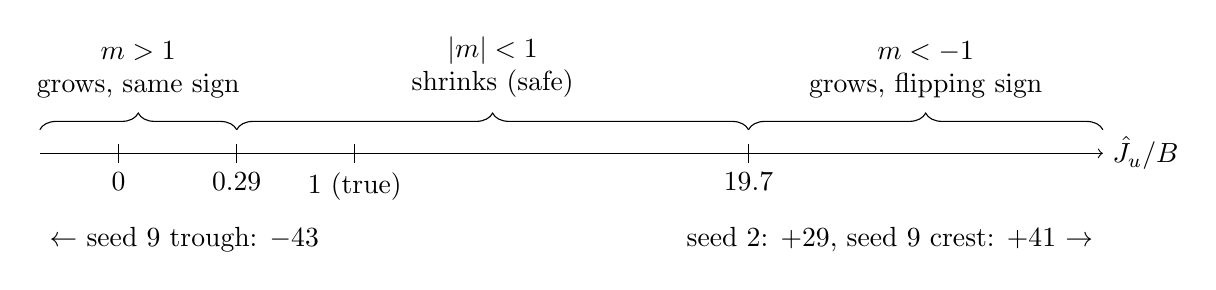
\begin{tikzpicture}[x=1cm,y=1cm]
\draw[->] (-1,0) -- (12.5,0) node[right] {$\hat J_u/B$};
\foreach \p/\l in {0/0, 1.5/0.29, 3/1 (true), 8/19.7} {\draw (\p,0.12) -- (\p,-0.12) node[below] {\l};}
\draw[decorate,decoration={brace,amplitude=6pt}] (-1,0.3) -- (1.5,0.3) node[midway,above=8pt,align=center] {$m>1$\\grows, same sign};
\draw[decorate,decoration={brace,amplitude=6pt}] (1.5,0.3) -- (8,0.3) node[midway,above=8pt,align=center] {$|m|<1$\\shrinks (safe)};
\draw[decorate,decoration={brace,amplitude=6pt}] (8,0.3) -- (12.5,0.3) node[midway,above=8pt,align=center] {$m<-1$\\grows, flipping sign};
\node[anchor=west] at (-1,-1.1) {$\leftarrow$ seed 9 trough: $-43$};
\node[anchor=east] at (12.5,-1.1) {seed 2: $+29$,\ seed 9 crest: $+41$ $\rightarrow$};
\end{tikzpicture}
\caption{Where the closed-loop multiplier shrinks or grows errors, as a function of the surrogate's input slope, for $\hat J_x=1.03$ and $K=10.29$. Not to scale. The true value $B$ sits safely inside; the kink's values fall on both sides.}
\end{figure}

\begin{center}
\begin{tabular}{lllllll}
\toprule
$\hat J_u/B$ & $-43$ & 0.29 & 1 & 19.7 & 29 & 41 \\
\midrule
$m=1.03-0.01\,(\hat J_u/B)\,10.29$ & 5.45 & 1.00 & 0.927 & $-1.00$ & $-1.95$ & $-3.19$ \\
\bottomrule
\end{tabular}
\end{center}

In words: if the surrogate says the input is too weak (or acts in the wrong direction), the controller cannot hold the slightly unstable plant in the surrogate's world, and errors grow ($m>1$). If the surrogate says the input is far too strong, the controller overshoots in the surrogate's world, and errors grow while flipping sign ($m<-1$). The kink produces both: input-slope peaks of 6.7 to 201 times $B$ and negative arms.

The lower edge is so close to zero because the plant is only slightly unstable ($A-1=0.03$), and the upper edge is set by the small input authority ($B=0.01$): a gain of 10 is needed, and a gain of 10 turns a 20-fold overestimate of $B$ into a full overshoot.

\subsection{An example: a kink on the way versus a kink at the destination}

Away from the kink the surrogate's slopes are close to the truth and the multipliers are safe. So one might expect the kink to spoil only a few multipliers, which the safe ones around them would absorb. Whether that happens depends on where the kink sits relative to the run. The example below uses made-up multipliers to show this; only the pattern matters.

Four runs of 200 steps. Every safe step has $m=0.9$. In runs B to D the run reaches the target at step 50 and stays there for the remaining 150 steps; since every LayerNorm kink centre lies within 0.1 of the origin, the target is inside the kink.
\begin{itemize}
\item Run A passes through the kink on its way elsewhere: 3 bad steps with $m=-3$ (steps 100 to 102), all other steps safe.
\item Run B lands in the kink, but the spot where it rests happens to have a right-signed, moderate input slope: all 150 steps there are safe ($m=0.8$).
\item Run C lands on a bad spot where 1 step in 25 has $m=-10$ (input slope far too large) and the rest are safe.
\item Run D lands on a bad spot where 1 step in 4 has $m=-10$ and the rest are safe.
\end{itemize}

\begin{figure}[H]
\centering
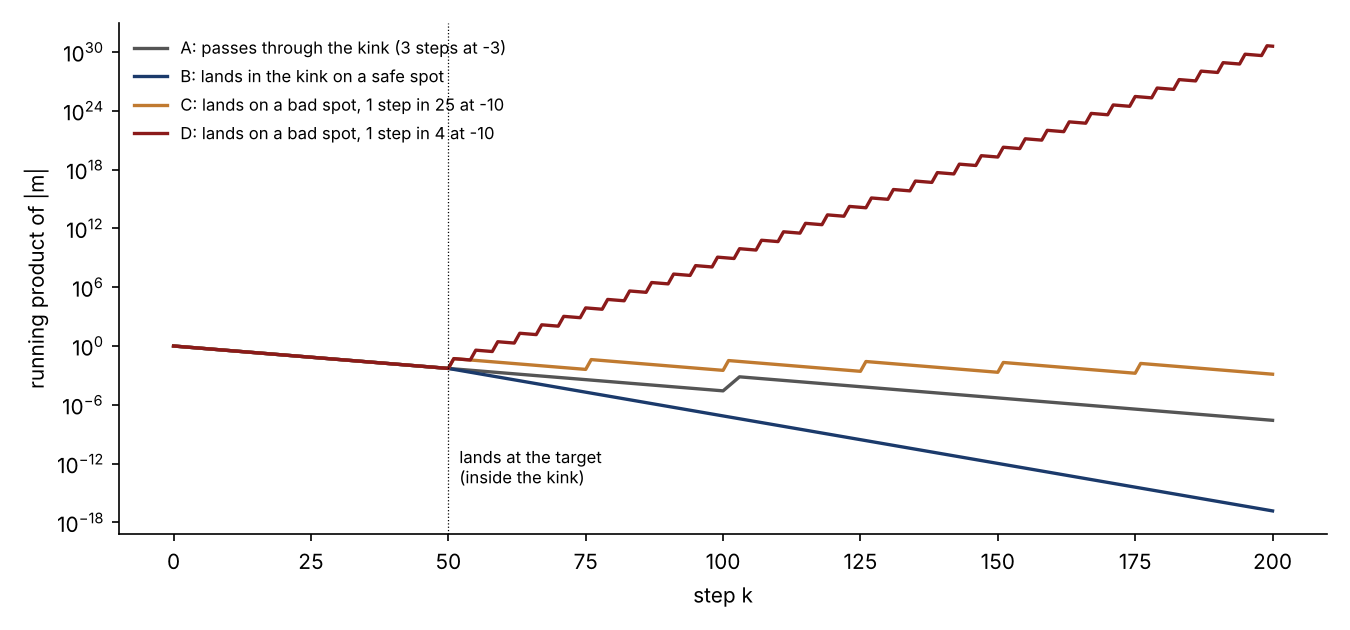
\includegraphics[width=0.9\textwidth]{fig_toy.png}
\caption{Running product of the multipliers' sizes for the four made-up runs (logarithmic axis). Up to step 50 all four are identical. Run D has 75 percent safe steps after landing and still explodes.}
\label{fig:toy}
\end{figure}

\begin{center}
\small
\begin{tabular}{lllllll}
\toprule
run & safe after & \multicolumn{3}{l}{running product at step} & worst & largest \\
 & landing & 100 & 150 & 200 & stretch & amplification \\
\midrule
A: passes through & 98\,\% & $3\times10^{-5}$ & $5\times10^{-6}$ & $3\times10^{-8}$ & 3.3 & 27 \\
B: safe spot & 100\,\% & $7\times10^{-8}$ & $10^{-12}$ & $2\times10^{-17}$ & 0 & 1 \\
C: 1 bad in 25 & 96\,\% & $3\times10^{-3}$ & $2\times10^{-3}$ & $10^{-3}$ & 2.3 & 10 \\
D: 1 bad in 4 & 75\,\% & $10^{9}$ & $2\times10^{19}$ & $4\times10^{30}$ & 75.8 & $8\times10^{32}$ \\
\bottomrule
\end{tabular}
\end{center}

What the example shows:
\begin{itemize}
\item Run A matches the intuition, and it is correct: a few bad steps on the way are absorbed. A deposit made just before them is amplified 27 times, then the safe steps shrink it again.
\item The difference between C and D is how often the bad steps come. One step with $|m|=10$ multiplies by 10; it takes 22 steps at 0.9 to divide by 10 again ($0.9^{22}\approx0.1$). In C there are 24 safe steps between bad ones, slightly more than 22, so the product drifts slowly down. In D there are only 3, so every block of four steps multiplies by $10\times0.9^3=7.3$, a typical multiplier of $e^{0.50}=1.64$ per step, for 150 steps.
\item The bad steps in C and D are not ``a few points along the way''. They recur for as long as the run stays at the target, and a regulation run stays there for the rest of the horizon.
\end{itemize}

How the real runs compare (Figure~\ref{fig:zones}, Section 13): LN MSE seed 2 and seed 8 are like run D, with 41 and 37 percent of their landing steps at $m\approx-10$ and $-4.4$, and a growth of 0.39 and 0.30 per step. The static-norm surrogate is like run B, with no bad spot at all. LN MSE seed 7 and LN MSE 12000 seed 2 are also like run B: their kinks are tall (23 and 35 times $B$ at the peak), but at the spot where the good controller rests the input slope is 6.2 and 4.9 times $B$, inside the safe band. Seed 1 is close to run C: its exponent is barely positive, only 1.6 percent of its starts have a growing product, and in the warm-start test (slide 19) its controller was kicked out and then returned.

So a DPC trap needs two things together: a target inside the kink, so that the run keeps sampling the kink's slopes for the rest of the horizon, and a resting spot where those slopes push the multiplier out of the safe band often enough.

\section{How the state can stay near zero while the derivative explodes}

This is the puzzling part of the slide: the state jitters within 0.05 of the target, yet its derivative reaches $10^{34}$.

Values and slopes are different properties of a function. A function can be close to another in value and far from it in slope. Example: $f(x)=x+0.001\sin(1000x)$ is never more than 0.001 away from $x$, but its slope $1+\cos(1000x)$ swings between 0 and 2 while the slope of $x$ is 1. The surrogate near the kink is like this: its values are close (errors of a few thousandths, up to a few hundredths right at the kink centre), so the rollout's states, and the cost computed from them, are about right; its input slope can be wrong by factors of tens to hundreds, so the multipliers $m_k$ and everything built from them are wrong.

Remember also that $\delta x_k$ is a ``what if'' quantity: the first-order response to an infinitely small nudge of the weights. It measures how sensitive the run is to the weights, not where the run goes. A run can stay near zero while being extremely sensitive to the weights, much as a ball rolling in a bumpy bowl always stays inside the bowl, while two balls started a hair apart soon end up in completely different places in it. Even multiplied by $x_k\approx0.03$ in the cost, a sensitivity of $10^{34}$ is enormous.

This is not the usual exploding gradient of backpropagation through an unstable system. The true closed loop is stable ($\lambda<0$); the instability exists only inside the surrogate, created by its wrong slopes.

\section{The GRU controller}

The DPC controller is a GRU, which also has a memory $h_k$ of 64 numbers: $u_k=\pi(x_k,h_k;\theta)$ and $h_{k+1}=g(x_k,h_k;\theta)$. Everything above still applies, with two changes. The balance is now a list of 65 numbers $(\delta x_k,\delta h_k)$ instead of one. The multiplier $m_k$ becomes a $65\times65$ table of numbers (a matrix), and multiplying by it means a matrix--vector product. The size of the balance is then measured by its length (norm), and $\lambda$ becomes the average log-growth of that length.

\section{Reading slide 17}

\subsection{The slide at a glance}

The slide has four parts:
\begin{enumerate}
\item the title, ``Why: through the kink, the gradient explodes'';
\item one formula, $\|\nabla L\|\sim e^{N\lambda}$, with $\lambda$ described as the closed-loop Lyapunov exponent of the rollout through the surrogate;
\item a figure with three panels;
\item three short statements under the figure.
\end{enumerate}
Its message in one sentence: the surrogate prices the good controller correctly, but its wrong slopes make the closed loop through it locally expanding, so the gradient that DPC would follow near the good controller is astronomically large, and DPC cannot settle there.

Its place in the talk: slide 16 showed that DPC through the narrow-kink surrogates fails, and that the surrogate itself rates the good controller correctly (an optimisation trap, not model mismatch). Slide 17 explains why the optimiser cannot reach the good controller. Slide 18 then shows that the exploding gradient also points in random directions, slide 19 that it pushes a controller out even when training starts at the good one, and slide 20 that replacing the surrogate's input slope by the true one removes the explosion.

\subsection{The experiment behind the figure}

No training happens in this figure. It was made in four steps.
\begin{enumerate}
\item Take the good controller: the GRU trained by DPC through the true plant (the oracle). Its cost on the true plant is 2.50, within 0.04 percent of the analytic LQR.
\item Pick a surrogate and one start. The start is the one that dominates that surrogate's gradient at the good controller: of the 1000 training starts, this single start carries about three quarters of the squared gradient norm on seed 2 and 99 percent on seed 8 (Section 13.10).
\item Run the good controller from that start for 200 steps twice: once through the true plant and once through the surrogate.
\item At every step record the state $x_k$ (dashed line) and the running product of the multipliers (solid lines), computed exactly by differentiating the run.
\end{enumerate}

Why the good controller? DPC would have to settle at a controller like this one. To settle somewhere, the gradient there must be small and smooth, so that the optimiser's steps shrink as it approaches. The figure checks whether that holds near the good controller, through each model.

\subsection{How to read the axes}

\begin{itemize}
\item Horizontal axis: the step $k$, from 0 to 200.
\item Left vertical axis (logarithmic): the running product of the multipliers. The slide writes it as $\|\partial(h_k,x_k)/\partial x_0\|$; Section 13.4 explains the notation. Each gridline is a factor $10^5$. Every curve starts at 1 at step 0.
\begin{itemize}
\item A falling curve means the multipliers are, on average, below 1 in size: old changes are forgotten.
\item A flat curve means they average exactly 1 in size.
\item A rising straight line means a steady typical multiplier above 1; its slope is $\lambda$ (Section 9.2).
\end{itemize}
\item Right vertical axis (linear, $-0.3$ to $0.3$): the state $x_k$ of the run through the surrogate, drawn dashed.
\item Black solid: through the true plant. Coloured solid: through the surrogate (green for static norm, orange for LayerNorm).
\end{itemize}

\subsection{Why the plot nudges the start rather than the weights}

The gradient needs the response to a change of the weights (Section 6), which mixes two things: the deposits $s_k$ and the multipliers $m_k$. The plot isolates the multipliers with a trick: it changes the start $x_0$ and keeps the weights fixed. Then no deposits are made ($s_k=0$); the account opens with balance $\delta x_0$ and is only multiplied:
\begin{equation}
\delta x_k=m_{k-1}\,m_{k-2}\cdots m_0\;\delta x_0,\qquad\text{so}\qquad \frac{\partial x_k}{\partial x_0}=m_{k-1}\,m_{k-2}\cdots m_0 .
\end{equation}
Each curve is therefore the running product of the multipliers along that run. Every deposit in the gradient is multiplied by a piece of this running product (Section 6.4), so when this curve explodes, the gradient explodes with it.

For the GRU the state includes the 64 memory units $h_k$, so the derivative is a list of 65 numbers, and the plot shows its length (norm). That is the meaning of $\|\partial(h_k,x_k)/\partial x_0\|$.

\subsection{Left panel: static norm, seed 2, start $x_0=-0.37$}

What you see: both solid curves fall together and almost coincide, and the dashed state settles near zero.

\begin{center}
\begin{tabular}{llll}
\toprule
step $k$ & 50 & 100 & 200 \\
\midrule
running product, true plant & 0.082 & 0.040 & 0.019 \\
running product, surrogate & 0.071 & 0.039 & 0.018 \\
\bottomrule
\end{tabular}
\end{center}

What the multipliers do: along this run the surrogate's input slope stays between 1.02 and 1.17 times $B$, and every step is in the safe zone (top row of Figure~\ref{fig:zones}). The state settles at $-0.025$ instead of 0, a small offset caused by the surrogate's value error, unrelated to the kink.

Why the decay is slower than $0.927^k$: the plotted length includes the GRU's memory units, which forget the start slowly; the plant state alone would forget it much faster.

Message: through a kink-free surrogate, the closed loop behaves like the true one, and the gradient at the good controller is small.

\subsection{Middle panel: LN MSE 3000, seed 2, start $x_0=+0.02$}

What you see: the run starts at the target and stays there, with the dashed state jittering between 0.018 and 0.055 for the whole run. The black curve falls as before. The orange curve rises along a roughly straight line by about 34 powers of ten.

\begin{center}
\begin{tabular}{llllll}
\toprule
step $k$ & 25 & 50 & 100 & 150 & 200 \\
\midrule
running product, true plant & -- & 0.073 & 0.030 & -- & 0.015 \\
running product, surrogate & $9.4\times10^3$ & $2.6\times10^{10}$ & $3.7\times10^{21}$ & $2.0\times10^{28}$ & $1.6\times10^{34}$ \\
\bottomrule
\end{tabular}
\end{center}

The slope of the orange line is about 0.39 per step, a typical multiplier of $e^{0.39}=1.48$: every step stretches the response by about half again, 200 times in a row.

What the multipliers do (middle row of Figure~\ref{fig:zones}). The run sits right at the kink centre ($x$ between 0.02 and 0.06, $u$ between $-1.2$ and $-0.1$), where a crest and a trough of the input slope lie side by side (slide 6). Small changes of $(x_k,u_k)$ from step to step move the operating point across them, so the surrogate's input slope jumps between about $-0.5\,B$ and $+90\,B$. Using the controller's direct gain (about 22 here), the steps fall into the three zones of Section 10 as follows:
\begin{itemize}
\item 41 percent of steps: input slope far too large (median $+50\,B$), multiplier about $-10$ (red);
\item 14 percent of steps: input slope slightly negative (median $-0.5\,B$), multiplier about $1.07$ (blue);
\item 44 percent of steps: safe (grey).
\end{itemize}
The safe steps cannot compensate: a single step with $|m|=10$ adds as much growth ($\log10=2.3$) as about 22 steps at 0.9 remove ($\log0.9=-0.105$ each).

Message: the state is fine and the cost is fine; only the derivative explodes. This is Section 11 in one picture.

\subsection{Right panel: LN MSE 3000, seed 8, start $x_0=+2.37$}

What you see: three phases.

\begin{center}
\small
\begin{tabular}{p{2.2cm}p{5.2cm}p{6.6cm}}
\toprule
steps & what the run does & what the curves do \\
\midrule
0 to about 35 & far from the target; the input is saturated at $-10$ & both curves rise together to about 40 at step 33 \\
about 35 to 75 & a normal landing towards zero, outside the kink & both curves fall together; at step 50 they are 1.81 (surrogate) and 1.75 (true) \\
from about 75 & the run reaches $x\approx0.01$ to $0.04$, inside the kink & the curves separate (ratio 2 at step 75, 10 at step 80); the surrogate's rises to 9.0 at step 100, $3.6\times10^7$ at 150 and $9.1\times10^{13}$ at 200; the true one ends at 0.027 \\
\bottomrule
\end{tabular}
\end{center}

The first-phase bump is not the kink. While the input is saturated, the controller's output does not respond to small changes ($K_k\approx0$), so the multiplier is just $\hat J_x\approx1.03$ (blue in the bottom row of Figure~\ref{fig:zones}), and the GRU's memory adds to the rise. It appears identically on both models, so it is a property of the controller, not of the surrogate.

In the third phase the multipliers look like those of seed 2: 37 percent of the landing steps have an input slope far too large (median $+27\,B$, multiplier about $-4.4$), 33 percent a wrong-signed one (median $-1.2\,B$, multiplier about $1.2$), 29 percent are safe. The growth is about 0.30 per step, a typical multiplier of $e^{0.30}=1.35$.

Message: the growth switches on exactly when the run enters the kink, and not before.

\begin{figure}[H]
\centering
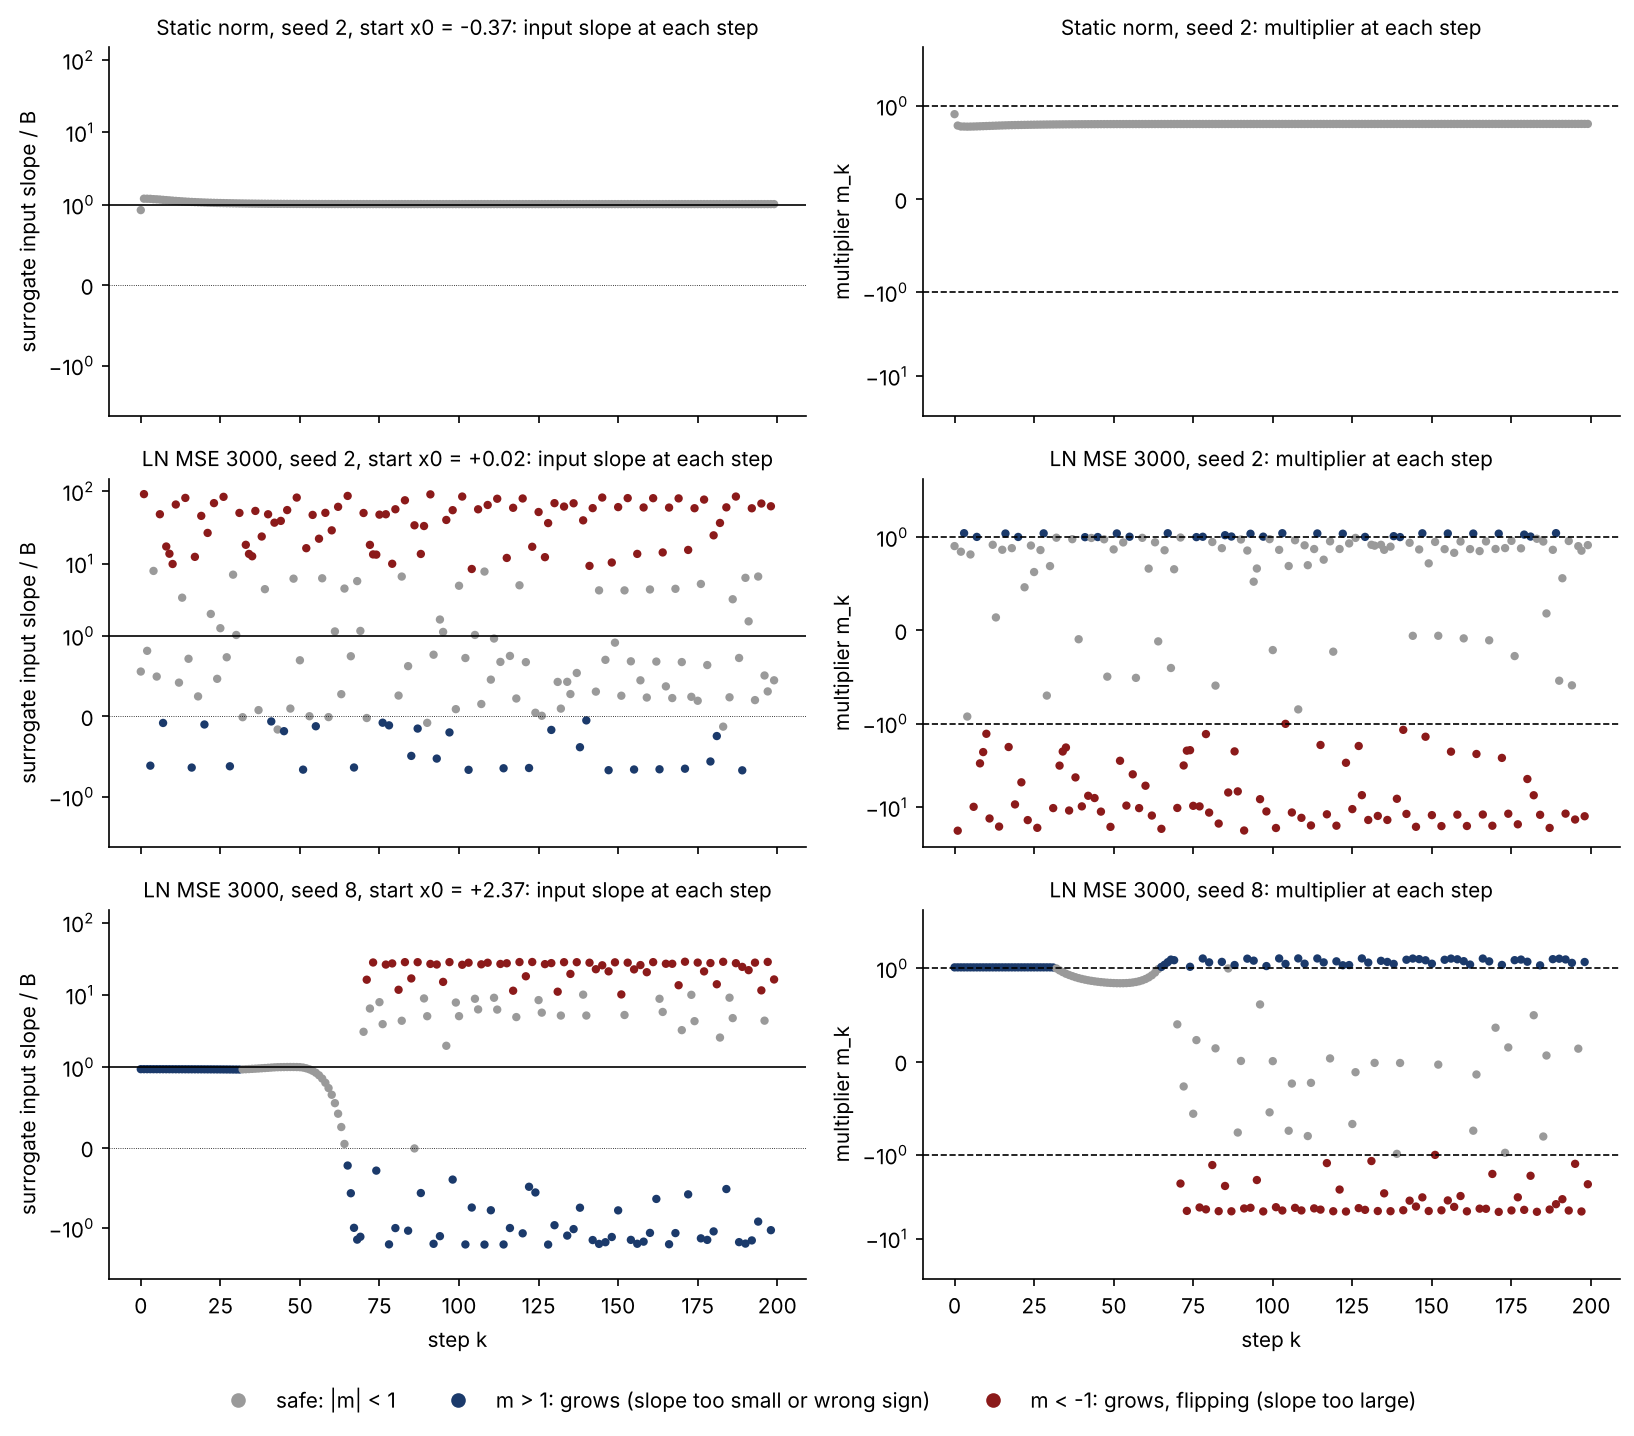
\includegraphics[width=\textwidth]{fig_zones.png}
\caption{What the multipliers do along the three runs of slide 17, one dot per step, coloured by zone. Left: the surrogate's input slope at $(x_k,u_k)$, divided by $B$ (true value 1, solid line). Right: the multiplier $m_k=\hat J_x-\hat J_u K_k$, with the GRU's direct gain $K_k=-\partial u_k/\partial x_k$ (memory held fixed); dashed lines at $\pm1$ bound the safe zone. Grey: safe. Blue: $m_k>1$ (input slope too small or wrong sign, or input saturated). Red: $m_k<-1$ (input slope too large). The colours match the kink maps, where red marks an overestimated and blue an underestimated or wrong-signed input slope. Logarithmic axes, linear between $-1$ and $1$. This scalar multiplier ignores the GRU's memory, so its numbers are indicative; the plot on slide 17 is exact.}
\label{fig:zones}
\end{figure}

\subsection{The formula, checked against the measurements}

Section 9.2 gives $|m_1\cdots m_N|=e^{N\lambda}$ exactly, and the gradient follows the products roughly: $\|\nabla L\|\sim e^{N\lambda}$. The table compares $e^{200\lambda}$ with the measured gradient at the good controller, from two independent computations.

\begin{center}
\begin{tabular}{lllll}
\toprule
broken pair (repeat 0) & $\lambda$ & $e^{200\lambda}$ & gradient, & gradient, \\
 & & & computation 1 & computation 2 \\
\midrule
LN MSE seed 1 & 0.012 & 11 & $1.3\times10^3$ & $1.3\times10^3$ \\
LN MSE seed 2 & 0.418 & $2\times10^{36}$ & $1.1\times10^{35}$ & $3.9\times10^{35}$ \\
LN MSE seed 8 & 0.157 & $4\times10^{13}$ & $3.1\times10^{13}$ & $9.2\times10^{13}$ \\
LN MSE seed 9 & 0.136 & $7\times10^{11}$ & $1.2\times10^{14}$ & $1.9\times10^{11}$ \\
slope from step 0, seed 2 & 0.211 & $2\times10^{18}$ & $2.7\times10^{24}$ & $4.9\times10^{18}$ \\
\bottomrule
\end{tabular}
\end{center}

How to read it:
\begin{itemize}
\item On seeds 2 and 8 the rule gives the right order of magnitude; these are the two checks quoted in the slide's notes.
\item On seed 9 and slope-from-step-0 seed 2, the two computations of the same gradient disagree by factors of 600 and $10^6$, and the rule falls inside that spread. Gradients this large cannot be computed reproducibly, because rounding errors are amplified by the same products. That is itself a symptom of the explosion.
\item On seed 1 the rule fails ($11$ against $1.3\times10^3$): its $\lambda$ is barely positive, and the gradient comes from a short burst of growth rather than steady growth. Section 14.3 replaces $\lambda$ by a quantity that captures bursts.
\end{itemize}
So the formula is an order-of-magnitude guide, not a prediction to several digits.

\subsection{Statement 1: $\lambda>0$ on 5 of the 6 broken pairs}

What was measured: for each surrogate, $\lambda=\frac1{200}\log\|\partial(h_{200},x_{200})/\partial x_0\|$ of the good controller, computed for 64 starts; the slide quotes the largest.

\begin{center}
\begin{tabular}{llll}
\toprule
pair & $\lambda$ & DPC failed? & note \\
\midrule
true plant & $-0.076$ & -- & $\log0.927$ \\
LN MSE seeds 1, 2, 8, 9 & 0.012, 0.418, 0.157, 0.136 & yes & positive \\
slope from step 0, seed 2 & 0.211 & yes & positive \\
slope from step 0, seed 9 & $-0.025$ & yes & the exception \\
every healthy pair, e.g.\ two-stage & $-0.02$ to $-0.07$ & no & negative \\
\bottomrule
\end{tabular}
\end{center}

The exception: slope-from-step-0 seed 9 is quiet at the good controller (gradient 0.55), but between the trapped controller and the good one its gradient spikes to $5\times10^{26}$. The trouble lies on the way in, not at the destination.

Caveat for questions: the sign of $\lambda$ alone is not the criterion. In repeats 1 and 2, seed 0 has a small positive $\lambda$ (0.029 and 0.017) and trains fine. What matters is how large the amplification gets, which is what Section 14.3 measures.

\subsection{Statement 2: the gradient at the good controller}

What was measured: the length of the gradient of the DPC loss (all 1000 starts) with respect to all 12\,737 GRU weights, at the good controller. On the broken pairs it is $10^3$ to $10^{35}$ (table in Section 13.8); on the healthy pairs of repeat 0 it is 0.03 to 3.5.

Why size alone is not the whole problem: the optimiser (Adam) rescales its steps, so a uniformly large gradient would be harmless. The problem is that the gradient is a single start's contribution, multiplied by an exploding product: on the broken pairs, one start carries 61 to 100 percent of the squared gradient norm, against at most 2 percent on healthy pairs. Its direction is set by that one run's multipliers, which change completely when the weights change by one part in $10^4$ (slide 18). So each step points in an essentially random direction.

\subsection{Statement 3: the loss value stays right}

What was measured: the cost of the good controller computed through each surrogate (the run of Section 13.2 for all 1000 starts), against its true cost of 2.50.

\begin{center}
\begin{tabular}{lll}
\toprule
 & \multicolumn{2}{l}{cost computed through the surrogate} \\
pair & good controller & DPC's own controller \\
\midrule
LN MSE seed 1 & 2.55 & 9.61 \\
LN MSE seed 2 & 2.51 & 8.53 \\
LN MSE seed 8 & 2.56 & 19.26 \\
LN MSE seed 9 & 2.48 & 1861 \\
slope from step 0, seed 2 & 2.47 & 4.33 \\
slope from step 0, seed 9 & 2.39 & 7.89 \\
\bottomrule
\end{tabular}
\end{center}

The surrogate's cost for the good controller is within 5 percent of the truth, and by its own numbers the good controller is 1.8 to 750 times better than what DPC found. Values right, slopes wrong (Section 11).

\subsection{The slide in three sentences, and common misreadings}

The surrogate's values are right, so it prices the good controller correctly. Its input slope near the kink is far too large or wrong-signed, so along a run that lands at the target the closed-loop multipliers keep leaving the safe zone, and their running product, which every gradient is built from, explodes. DPC needs a small, smooth gradient near the good controller to settle there, and it does not get one.

Common misreadings:
\begin{itemize}
\item ``The surrogate's trajectory diverges.'' No: the state stays within 0.06 of the target.
\item ``Backpropagation through 200 steps always explodes.'' No: through the true plant the same products decay.
\item ``Only the wrong-signed input slope matters.'' No: on seeds 2 and 8 the largest multipliers come from an input slope that is far too large (red steps).
\item ``$\lambda>0$ means DPC will fail.'' Not exactly: small positive values occur without failure; the size of the amplification decides.
\item ``The gradient sizes are precise.'' No: only their order of magnitude is reproducible.
\end{itemize}

\section{What the theory work added}

\subsection{Why go further than the slide}

The slide's account has three weak points, visible in Section 13: the formula $e^{N\lambda}$ is only an order-of-magnitude guide; the sign of $\lambda$ does not decide failure (seed 0, repeats 1 and 2); and one broken pair has a quiet good controller (slope-from-step-0 seed 9). The theory work (Theorem 2 of the theory note, 28 October) asked which multipliers, where, and how many, and turned the answer into a test that can be run on any surrogate before DPC training.

\subsection{Both edges of the safe band matter}

Section 10 derived the safe band for the LQR gain, $0.29\,B<\hat J_u<19.7\,B$. The GRU acts with a direct gain of 13 to 22 at landing, about twice the LQR gain, which narrows the band: with $K=20$ it becomes about $0.15\,B<\hat J_u<10\,B$. Figure~\ref{fig:zones} shows the consequence on seeds 2 and 8: most growing steps lie above the band (red), from an input slope 25 to 90 times too large, not below it. An overestimated input slope explodes the gradient as surely as a wrong-signed one. This differs from the LQR half of the talk, where the catastrophic failures came from wrong-signed (blue) setpoint slopes.

\subsection{The landing amplification $\Lambda^\star$}

The average $\lambda$ over the whole run can hide a short burst of growth: a burst of 40 steps with typical multiplier 1.5 amplifies a deposit made at its start by $1.5^{40}\approx10^7$, even if the other 160 steps shrink things and the average is near zero. The theory therefore looks at the worst stretch instead of the average.

How $\Lambda^\star$ is computed, for the good controller and one surrogate:
\begin{enumerate}
\item For each of the 1000 starts, run the good controller through the surrogate and compute $\log|m_k|$ at every step.
\item Keep only the landing: from the first step with $|x_k|\le0.2$ to the end.
\item Find the stretch of consecutive steps whose $\log|m_k|$ add up to the largest total. Call this total $\Lambda$ for that start. Then $e^{\Lambda}$ is the largest amplification any deposit can receive during that landing.
\item $\Lambda^\star$ is the largest $\Lambda$ over the 1000 starts.
\end{enumerate}

Example for step 3, with seven steps whose $\log|m_k|$ are $-0.1,\ 0.5,\ 0.7,\ -0.2,\ 0.6,\ -1.0,\ 0.3$. The best stretch is steps 2 to 5: $0.5+0.7-0.2+0.6=1.6$, an amplification of $e^{1.6}\approx5$. Extending it further only lowers the total (adding $-1.0$ and $0.3$ gives 0.9), and starting earlier adds $-0.1$. Note that a stretch may include a few shrinking steps, as long as the steps around them more than make up for it.

The threshold: the largest $\Lambda^\star$ among the 18 healthy LN MSE 3000 runs is 8.6, the smallest among the 12 trapped ones is 17.0, and the threshold is set between them at 12.1 (their geometric mean), an amplification of about $2\times10^5$. It was fixed on LN MSE 3000 and then applied unchanged to the other five families.

\begin{figure}[H]
\centering
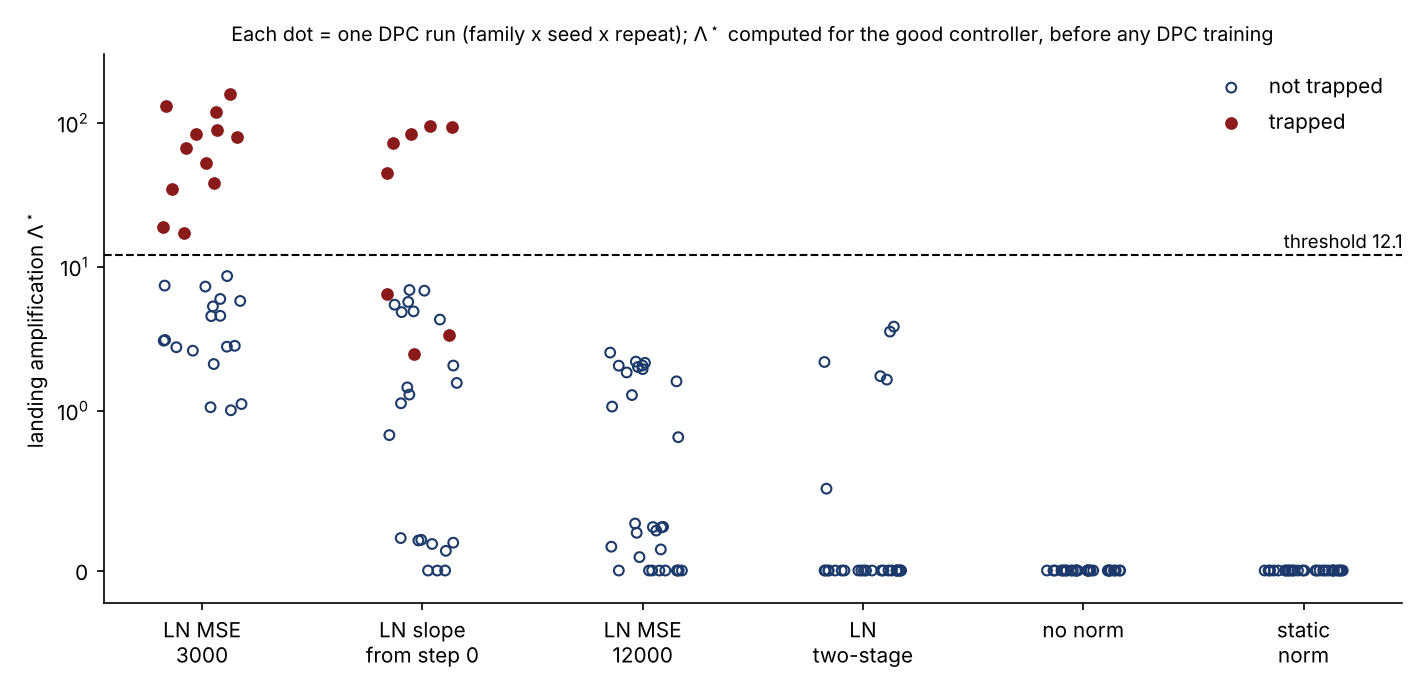
\includegraphics[width=\textwidth]{fig_lambda.png}
\caption{Landing amplification $\Lambda^\star$ of the good controller through each surrogate, for all 180 DPC runs (6 families, 10 seeds, 3 repeats). Filled red: runs where DPC was trapped. Open blue: all other runs. Dashed: the threshold 12.1. Logarithmic axis, linear between 0 and 1; a value of 0 means no stretch of the landing grows at all.}
\label{fig:lambda}
\end{figure}

\begin{center}
\begin{tabular}{lllll}
\toprule
family & runs & trapped & trapped and flagged & flagged but not trapped \\
\midrule
LN MSE 3000 & 30 & 12 & 12 & 0 \\
LN slope from step 0 & 30 & 8 & 5 & 0 \\
LN MSE 12000 & 30 & 0 & -- & 0 \\
LN two-stage & 30 & 0 & -- & 0 \\
no norm & 30 & 0 & -- & 0 \\
static norm & 30 & 0 & -- & 0 \\
\midrule
all & 180 & 20 & 17 & 0 \\
\bottomrule
\end{tabular}
\end{center}

The three missed traps are all slope-from-step-0 runs (seed 4 repeat 1, seed 9 repeat 1, seed 3 repeat 2) with $\Lambda^\star$ between 2.5 and 6.5: like seed 9 on the slide, their trouble lies away from the good controller. For comparison, the simpler tests catch fewer: a gradient above $10^3$ at the good controller flags 14 of the 20 traps, and $\lambda>0$ flags 16 of them but also 6 runs that were not trapped. On every one of the 180 runs the gradient at the good controller is at most $4.7\,e^{\Lambda^\star}$, so $\Lambda^\star$ also bounds the gradient from above, which $e^{N\lambda}$ did not reliably do. The bound also holds on the 90 linear runs computed and on 89 of 90 MLP runs (one at 6.1); the factor 4.7 was read off the GRU runs, and the linear and MLP gradients were computed on three of the six families (30 runs each). It is an upper bound, not an estimate: of the 28 GRU runs with $\Lambda^\star>5$ the gradient is within a factor $10^3$ of it on 8. The separation of traps above is retrospective: the threshold was fitted on these runs.

\subsection{The swap along the same runs}

The theory repeated the $\Lambda^\star$ computation with one of the surrogate's slopes replaced by the true value, along the same runs. Replacing the input slope by $B$ brings $\Lambda^\star$ below the threshold on 9 of the 12 LN MSE traps (to at most 5.7). Replacing the state slope by $A$ does so on none. In the three remaining cases (seed 9 in repeats 1 and 2, seed 1 in repeat 2) the state slope alone also expands: with the true input slope and a gain of 20 the multiplier is $\hat J_x-0.2$, which exceeds 1 where the state-slope crest passes 1.2. This is the run-by-run version of slide 20.

\subsection{Height is not enough; what the landing crosses decides}

Two seeds with almost the same peak input-slope error behave oppositely: seed 1 (24.4 $B$) is trapped in all 3 repeats, seed 7 (23.1 $B$) in none. LN MSE 12000 seed 2 has an even taller peak (35.5 $B$) and $\Lambda^\star$ between 2.0 and 2.6 in its three repeats. A tall kink only traps DPC if the good controller's landing passes through the parts of it that leave the safe band, which depends on where the crest and the arms lie relative to the landing.

\subsection{The controller's memory matters}

The same test for a memoryless controller, the saturated LQR $u=10\tanh(-K^\star x/10)$, gives $\Lambda^\star\le8.7$ on all 180 runs: below the threshold everywhere. Two features of the GRU make it vulnerable. Its direct gain at landing (13 to 22) is about twice the LQR gain, which narrows the safe band (Section 14.2). And its landing orbit moves: on seed 2, repeat 0, its input drifts from $-1.6$ to $-0.07$ during the landing, sweeping the crest and the arms. Prediction, made before the runs: a linear DPC controller would not be trapped, and the MLP's own good controller decides for the MLP. Outcome:
\begin{itemize}
\item The linear controller was never trapped. But its trained good controller (gain about 17) expands up to $e^{93}$ on 12 runs, and those were false alarms.
\item The MLP was trapped on 40 runs, none of them flagged: its good controller stays below the threshold ($\Lambda^\star\le7.4$).
\end{itemize}

\subsection{What is proved and what is a statistic}

For a memoryless controller, Theorem 2 is exact: the gradient is built from the multipliers as in Section 6, and an expanding stretch of length and strength $\Lambda$ forces the gradient up by about $e^{\Lambda}$. For the GRU, the multiplier with the direct gain ignores the memory, so $\Lambda^\star$ is a statistic suggested by the theorem rather than a consequence of it. Its record above (17 of 20 traps, no false alarm) is a retrospective fit. In three pre-registered prospective tests it failed: MLP 0 of 40 traps flagged, linear 12 false alarms, GRU at $B=0.1$ 1 of 7 traps flagged. What it reliably gives is an upper bound on the gradient at the good controller, not its size. A trap also needs a tame region for the policy to settle in, which $\Lambda^\star$ does not see.

\subsection{What this suggests for slide 17}

Optional updates, if the talk is revised:
\begin{itemize}
\item In the notes, write the multiplier as $\hat J_x-\hat J_uK$ (the convention $u=-Kx$ of the LQR slides) and add that both too-large and wrong-signed input slopes leave the safe band.
\item Keep $\lambda$ for the intuition. Quote $\Lambda^\star$ as an upper bound on the gradient at the good controller (180 of 180 GRU runs, 90 of 90 linear, 89 of 90 MLP) and as a retrospective separation of the GRU traps (17 of 20, no false alarm in 160, threshold fitted on these runs). Not as a trap predictor: it failed three prospective tests.
\item Quote the gradient sizes as orders of magnitude only.
\end{itemize}

\section{The dashed and the solid lines of slide 17, once more}

Each panel of slide 17 is one run of the good controller from one start, done twice: once with the true plant and once with the surrogate playing the plant.

The dashed line is the state $x_k$ of the run through the surrogate, read on the right-hand axis. It says where the run actually went: in the middle panel it jitters between 0.02 and 0.055 for all 200 steps; in the right panel it comes down from 2.37, drops off the top of the axis, and sits near 0.02 from step 75 on. It makes one point: the run is well behaved, and the cost computed from these states is right.

The solid coloured line is not about where the run went. It answers a what-if question: had the start been nudged by a tiny amount, how much bigger would the difference be at step $k$? That is the running product $m_0 m_1\cdots m_{k-1}$ of Section 6 (with the GRU's memory included). It starts at 1 because at step 0 the difference is the nudge itself; it falls while the steps shrink differences and rises while they stretch them. In the middle panel it reaches $10^{34}$: a nudge of $10^{-34}$ at the start would be a difference of order 1 by step 200. The black line is the same what-if quantity for the run through the true plant, so one can see what normal looks like.

Every piece of the training gradient is a deposit multiplied by a stretch of exactly this product (Section 6.4). So where the solid line explodes, the gradient explodes with it, although the dashed line stays flat. Dashed: what happened. Solid: how sensitive what happened is.

\section{Slide 18: no barrier, a chaotic gradient, carried by one start}

\subsection{The question}
Slide 16 showed that DPC settles at a bad controller although the surrogate rates the good one as much better. The natural explanation is a hill in the loss between the two, with the optimiser stuck in a valley. Slide 18 tests that and rejects it.

\begin{figure}[H]
\centering
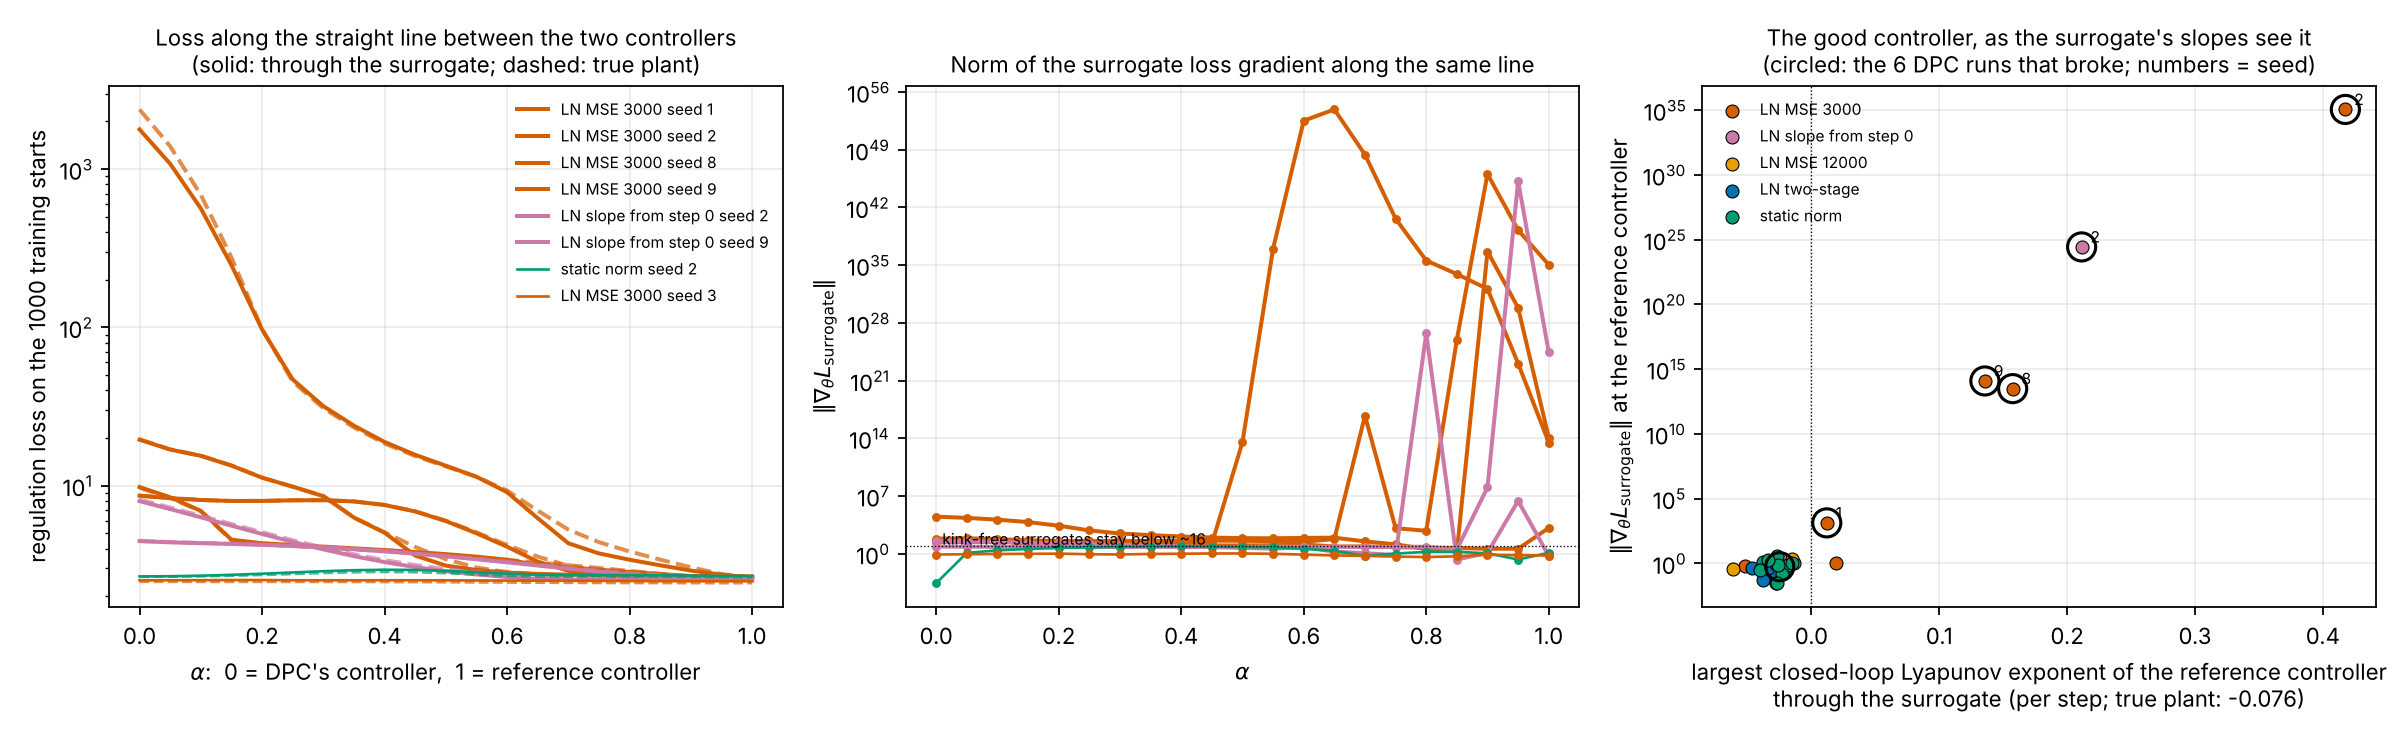
\includegraphics[width=\textwidth]{figP9_trap_landscape.png}
\caption{The figure on slide 18. Left: loss along the straight line from DPC's trapped controller ($\alpha=0$) to the good controller ($\alpha=1$), through the surrogate (solid) and the true plant (dashed). Middle: length of the surrogate loss gradient along the same line. Right: gradient length at the good controller against the Lyapunov exponent of slide 17; circled, the six DPC runs that broke.}
\end{figure}

\subsection{Left panel: walking from the bad controller to the good one}
Take DPC's trapped weights $\theta_{\rm bad}$ and the good controller's weights $\theta_{\rm good}$ and form the straight line $\theta(\alpha)=(1-\alpha)\theta_{\rm bad}+\alpha\theta_{\rm good}$. For 21 values of $\alpha$, evaluate the surrogate's DPC loss and the true-plant cost on the 1000 training starts. A hill would show as a rise before the fall. There is none: on all six broken pairs the loss falls monotonically from the trapped value (8 to 1800) to the good value (about 2.6). The trapped controller is not a flat point either: the gradient there has length 7 to 32\,000, so a descent method standing there sees a downhill direction and still does not take it.

\subsection{Middle panel: the gradient along the same line}
At the same 21 points, the length of the gradient of the surrogate loss. Kink-free surrogates and the healthy LN seed 3 stay below about 16 everywhere. The broken pairs spike to $10^{14}$ to $10^{54}$ between $\alpha=0.5$ and 1, near the good controller. This is the explosion of slide 17 seen along a path: it is a property of a whole region around the good controller, not of one point. Over all 30 LN MSE 3000 runs (three repeats), the largest gradient along this line is at least $10^3$ for every failed run and at most $10^2$ for every healthy one.

\subsection{Right panel: gradient size against $\lambda$}
One dot per surrogate and seed: horizontally the Lyapunov exponent of slide 17, vertically the gradient length at the good controller. Healthy pairs cluster at $\lambda<0$ and gradient about 1. Of the six circled broken runs, five sit at $\lambda>0$ with gradients $10^3$ to $10^{35}$; the sixth, slope-from-step-0 seed 9, has a quiet endpoint and its spike at $\alpha\approx0.8$ in the middle panel, on the way in.

\subsection{Carried by one start}
The DPC loss is averaged over 1000 starts, so its gradient is the average of 1000 per-start gradients. Measuring each start's share of the squared gradient length: on healthy pairs the largest share is 0.2 to 1.7 percent, a genuine average; on broken pairs one start holds 61 to 100 percent (seed 8: 99.9, seed 9: 99.96). It is the start whose landing lingers longest in the kink, and its exploded product swamps the other 999. The batch gradient is numerically the gradient of one trajectory.

\subsection{Chaotic}
Multiply every weight of the good controller by $1+10^{-4}\xi$ with random $\xi$, recompute the gradient, and take the cosine of the angle between the two gradients. Healthy pairs: 1.000, a smooth field. Broken pairs: $-0.15$, $-0.34$, $-0.07$ and the like; the direction is rerandomised by a change smaller than one Adam step (learning rate $10^{-3}$). Adam normalises step sizes, so a large gradient alone would be harmless; a large gradient whose direction is random at every step is what prevents convergence.

\subsection{Together}
No valley and no hill. Approaching the good controller the gradient becomes enormous, is carried by one trajectory, and points in a random direction. Gradient descent cannot enter that region and settles where the gradient is tame, which is the bad controller outside the kink. Open, and said on the slide: three slope-from-step-0 failures show no spike on the straight line; their spike presumably lies along the actual training path, which is not straight.

\section{Slide 19: start training at the good controller}

\subsection{Why an intervention}
Slides 17 and 18 measure a gradient field and predict that DPC cannot stay near the good controller. The direct test is to put the optimiser there and watch. If the explanation is right, plain gradient training pushes it out; if the traps were bad luck of initialisation, it stays.

\begin{figure}[H]
\centering
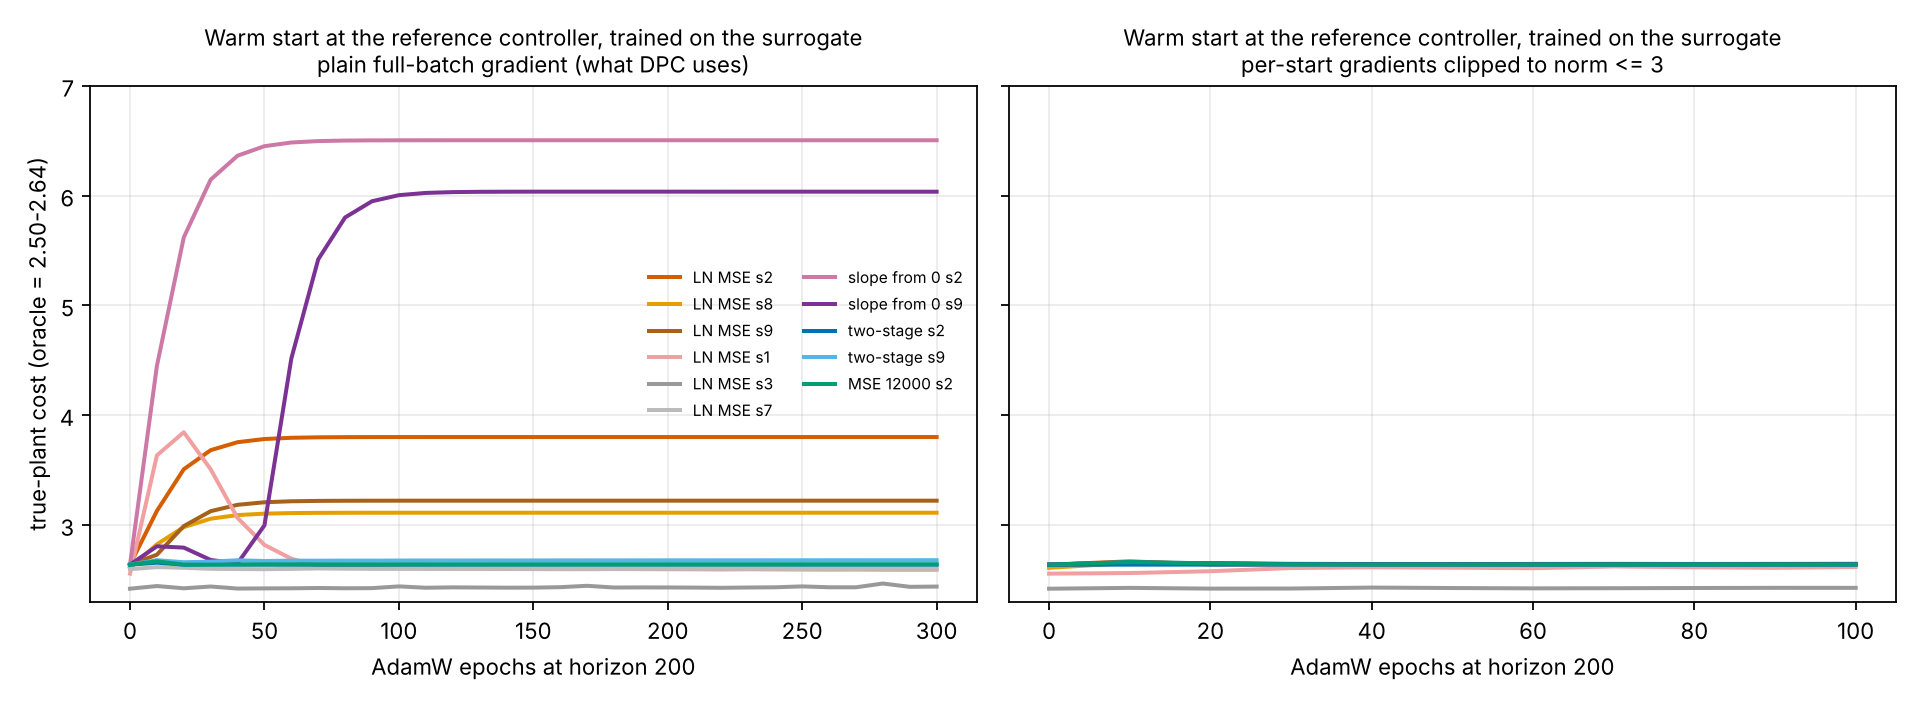
\includegraphics[width=\textwidth]{figP10_warmstart.png}
\caption{The figure on slide 19. AdamW started at the good controller and trained on each surrogate's own DPC loss at horizon 200 on its 1000 training starts; vertical axis, the true-plant cost after each epoch (oracle 2.50 to 2.64). Left: the plain full-batch gradient that DPC uses. Right: each start's gradient clipped to length at most 3 before averaging.}
\end{figure}

\subsection{Left panel: the plain gradient}
Healthy pairs (LN MSE seeds 3 and 7, two-stage seeds 2 and 9, MSE 12000 seed 2) stay at the oracle cost: a good controller stays good. On the broken pairs the cost rises within tens of epochs and plateaus: LN MSE seed 2 at 3.8, seed 8 at 3.1, seed 9 at 3.2, slope-from-step-0 seeds 2 and 9 at 6.5 and 6.0. Seed 1, the mildest trap, is kicked to 4.0 at epoch 10 and returns. The telling detail is that the surrogate's own loss rises too (seed 2 from 2.65 to 3.70, slope-from-step-0 seed 9 from 2.52 to 5.77): an optimiser walking uphill on its own objective, which is what the cosine test of slide 18 predicts. Training leaves a place where the loss is lower for one where it is higher.

\subsection{Right panel: per-start clipping}
Same experiment with one change in how the 1000 per-start gradients are combined: each is first shrunk to length at most 3, just above the healthy maximum, and then they are averaged. The exploding start now votes with weight 3 instead of $10^{35}$. Every pair, broken or healthy, stays at the oracle cost within 0.03, and the surrogate loss within 0.05 of its start.

\subsection{What the two panels prove}
Same surrogate, same starts, same loss, same optimiser; the only difference is whether one trajectory may dominate the batch. With domination the good controller is expelled, without it it stays. So the cause is the few exploding per-trajectory gradients, not the loss landscape and not the model's predictions. The clipping is a diagnosis rather than the proposed fix: it needs one to know that the explosion exists and to choose a threshold from the healthy scale, and it has not been run from a random initialisation (that run is pending). The proposed fix is two-stage training, which removes the kink at the source (slides 20 and 21). Also not run: global clipping of the averaged gradient, which the notes expect not to help, since the direction would still be set by the one start. Appendix slide A3 animates the same warm start with every start's gradient length plotted against its $x_0$: at epoch 0 one start sits at $10^{15}$ to $10^{38}$ while the rest sit below 3.

\end{document}
